\lecture{12}{27. April 2026}{The De Saint Venant Problem, Pt. III}

\subsection{Torsion of Circular Sections}
We consider a straight cylinder loaded by a torsional moment about its longitudinal axis, $M_3$ as shown on \Cref{fig:dsv2}. 

\begin{figure} [ht]
  \centering
  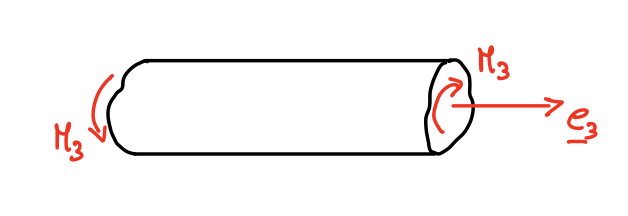
\includegraphics[width=0.8\linewidth]{./figures/dsv2.png}
  \caption{Torsionally-loaded straight bar}
  \label{fig:dsv2}
\end{figure}

We restrict our attention to circular cross sections, which are either solid circular shaft, hollow circular shafts, and thin circular tubes.
Circular sections are special because they do not warp under torsion, i.e. the cross-section remains a plane rigid disk under rotation.

Each cross-section rotates by an angle $\theta(x_3)$ around $e_3$.
The twist rate is
\begin{equation*}
  \theta' = \frac{\mathrm{d}\theta}{\mathrm{d}x_3} 
.\end{equation*}
If the torsion is uniform, $\theta'$ is constant, so
\begin{equation*}
  \theta(x_3) = \theta' x_3
.\end{equation*}

A point in the cross-section has position vector:
\begin{equation*}
  \Vec{r}(x_1, x_2) = \begin{pmatrix}
    x_1\\
  x_2\\
  0\\
  \end{pmatrix}
.\end{equation*}
For a small rotation $\theta(x_3)$ around $e_3$, the displacement is
\begin{equation*}
  \Vec{u}(x_1,x_2,x_3) = \theta(x_3) \Vec{e}_3 \times \Vec{r}(x_1, x_2)
.\end{equation*}
The cross product is then:
\begin{equation*}
  \Vec{e}_3 \times \Vec{r} = \begin{pmatrix}
    0\\
  0\\
  1\\
  \end{pmatrix} \times \begin{pmatrix}
    x_1\\
  x_2\\
  0\\
  \end{pmatrix} = \begin{pmatrix}
    -x_2\\
  x_1\\
  0\\
  \end{pmatrix}
.\end{equation*}
So
\begin{equation*}
  \Vec{u} = \theta' x_3 \begin{pmatrix}
    - x_2\\
  x_1\\
  0\\
  \end{pmatrix}
.\end{equation*}
Hence,
\begin{align*}
  u_1 &=  - \theta' x_3 x_2 \\
  u_2 &= \theta' x_3 x_1 \\
  u_3 &= 0
.\end{align*}
As $u_3 = 0$, there is no warping; points only move around the shaft axis and not up or down the shaft axis.

\subsubsection{Strains Produced by Torsion}
The only nonzero engineering shear strains are:
\begin{align*}
  \gamma_{31} &= - \theta' x_2 \\
  \gamma_{32} &= \theta' x_1
.\end{align*}
Using the linear elastic shear stress relation we obtain,
\begin{equation*}
  \tau = G \gamma
\end{equation*}
where $G$ is the shear modulus.
We get:
\begin{align*}
  \tau_{31} &= - G \theta' x_2 \\
  \tau_{32} &= G \theta' x_1
.\end{align*}
So the shear stress vector in the cross-section is:
\begin{equation*}
  \Vec{\tau}_3 = \begin{pmatrix}
    \tau_{31}\\
  \tau_{32}\\
  \\
  \end{pmatrix} = G \theta' \begin{pmatrix}
    -x_2\\
  x_1\\
  \\
  \end{pmatrix}
.\end{equation*}
This means the shear stress is tangent to circles around the center, with magnitude:
\begin{equation*}
  \left| \Vec{\tau}_3 \right| = G \theta' r
.\end{equation*}

We should note that
\begin{equation*}
  \mathrm{curl} \,  \Vec{\tau}_3 = 2 G \theta' \Vec{e}_3
.\end{equation*}
This comes from the field
\begin{equation*}
  \Vec{\tau}_3 = \begin{pmatrix}
    - G \theta' x_2\\
  G \theta' x_1\\
  \end{pmatrix}
.\end{equation*}
Two two-dimensional curl is
\begin{equation*}
  \frac{\partial \tau_{32}}{\partial x_1}  - \frac{\partial \tau_{31}}{\partial x_2} 
.\end{equation*}
Substituting, we obtain:
\begin{equation*}
  \frac{\partial }{\partial x_1} \left( G \theta' x_1 \right) - \frac{\partial }{\partial x_2} \left( - G \theta' x_2 \right) = G \theta' + G \theta' = 2G\theta'
.\end{equation*}
So the shear field circulates around the center.

\subsubsection{Torsional Moment for a Circular Section}
The torsional moment about $e_3$ is
\begin{equation*}
  M_3 = \int_A \left( \tau_{32}x_1 - \tau_{31}x_2 \right) \, \mathrm{d}A
.\end{equation*}
Substituting $\tau_{31}$ and $\tau_{32}$ we get:
\begin{equation*}
  M_3 = \int_A \left( G \theta' x_1^2 + G \theta' x_2^2\right) \, \mathrm{d}A
.\end{equation*}
So
\begin{equation*}
  M_3 = G \theta' \int_A \left( x_1^2 + x_2^2 \right)\, \mathrm{d}A
.\end{equation*}
Here, the integral
\begin{equation*}
  J = \int_A r^2 \, \mathrm{d}A = \int_A \left( x_1^2 + x_2^2 \right) \, \mathrm{d}A
\end{equation*}
is the polar second moment of area.
Hence,
\begin{equation*}
  M_3 = GJ\theta'
.\end{equation*}
So the torsional rigidity is:
\begin{equation*}
  C_T = GJ = \frac{M_3}{\theta'}
.\end{equation*}
This is the torsional equivalent of bending rigidity $EI$.

\subsubsection{Thin-Walled Sections and the Hydrodynamic Analogy}
The torsion equations are:
\begin{gather*}
  \mathrm{div}\, \Vec{\tau}_3 = 0 \quad \text{in }B \\
  \mathrm{curl} \,  \Vec{\tau}_3 = 2 G \theta' \quad \text{in } B \\
  \Vec{\tau}_3 \cdot \Vec{n} = 0 \quad \text{on } \partial B
.\end{gather*}
The last condition means the shear stress is tangent to the boundary; i.e. it cannot flow through the wall.

We can compare this to a fluid in a rotating container:
\begin{gather*}
  \mathrm{div}\,  \Vec{v} = 0 \\
  \mathrm{curl} \, \Vec{v} = \omega \Vec{e}_3 \\
  \Vec{v} \cdot \Vec{n} = 0
.\end{gather*}
So, the shear stress field behaves mathematically like a circulating velocity field, with streamlines corresponding to stress lines.

For a thin-walled section we describe the wall using $s$, as our coordinate along the mid-line, $\delta(s)$ as our wall thickness, $L$ as the total length of the mid-line, $t$ as the tangent direction along the wall and $n$ as a normal direction through the thickness.

The wall is thin, so
\begin{equation*}
  \delta(s) \ll L
.\end{equation*}
A point on the wall is describes uding
\begin{gather*}
  s \in \left[ 0, L \right] \\
  n \in \left[ - \frac{\delta(s)}{2}, \frac{\delta(s)}{2} \right]
.\end{gather*}
The stress components in the local frame are then $\tau_{zs}$ which is a shear stress along the wall tangent and $\tau_{zn}$ which is a shear stress through the wall thickness.

The boundary condition on the inner and outer wall surface is:
\begin{equation*}
  \tau_{zn} = 0 \qquad \text{at }n = \pm \frac{\delta(s)}{2}
.\end{equation*}
I.e. no shear stress flows through the free surface of the wall.

The exact curl equation is
\begin{equation*}
  \frac{\partial \tau_{zs}}{\partial n} - \frac{\partial \tau_{zn}}{\partial s} = 2 G \theta'
.\end{equation*}
Because the wall is thin and $\tau_{zn} = 0$ on both wall surfaces, we approximate $\tau_{zn}\approx 0$ throughout the thickness.
Then the equation becomes
\begin{equation*}
  \frac{\partial \tau_{zs}}{\partial n}  = 2G \theta'
.\end{equation*}
Integrating across the thickness yields:
\begin{equation*}
  \tau_{zs}(n) = 2G\theta' n + \tau_{zs}(0)
.\end{equation*}
So $\tau_{zs}$ varies linearly across the thickness.
But because $\delta(s) \ll  L$, the variation $2 G \theta' n$ is small compared to the mean tangential shear stress.
Therefore, we approximate the stress by its mean value across the thickness:
\begin{equation*}
  \tau_{zs}(n) \approx \overline{\tau}_{zs}
.\end{equation*}

\subsubsection{Shear Flow}
We now introduce the shear flow
\begin{equation*}
  q = \tau_z (s) \delta(s)
\end{equation*}
where $\tau_z$ is the average shear stress along the wall and $\delta(s)$ is the wall thickness.
So $q$ is force per unit length along the wall.

For a thin-walled closed section, the hydrodynamic analogy tells us that the shear flow is constant around the closed section, $q = \text{constant}$.
Therefore,
\begin{equation*}
  \tau_z(s) = \frac{q}{\delta(s)}
.\end{equation*}
So thinner parts of the wall carry higher shear stress.

\subsubsection{First Bredt Formula}
The small force on a wall element is
\begin{equation*}
  \mathrm{d}\Vec{F} = \tau_z(s) \Vec{t} \delta(s) \, \mathrm{d}s
.\end{equation*}
Since
\begin{equation*}
  q = \tau_z(s) \delta(s)
\end{equation*}
we can write
\begin{equation*}
  \mathrm{d}\Vec{F} = q \Vec{t} \, \mathrm{d}s
.\end{equation*}
The moment of this force about the origin is
\begin{equation*}
  \mathrm{d}\Vec{M}_t = \Vec{r} \times q \Vec{t} \, \mathrm{d}s
.\end{equation*}
Integrating about the mid-line yields:
\begin{equation*}
  \Vec{M}_T = \int_{\partial A_m} \Vec{r} \times \Vec{t} q \, \mathrm{d}s
.\end{equation*}
Since $q$ is constant,
\begin{equation*}
  \Vec{M}_t = q \int_{\partial A_m} \Vec{r} \times \Vec{t} \, \mathrm{d}s
.\end{equation*}
Taking the scalar component along $e_3$, gives
\begin{equation*}
  M_t = q \int_{\partial A_m} \left( \Vec{r} \times \Vec{t} \right) \cdot \Vec{e}_3 \, \mathrm{d}s = q \int_{\partial A_m} \Vec{r} \cdot \Vec{n} \, \mathrm{d}s
.\end{equation*}
By the divergence theorem,
\begin{equation*}
  \int_{\partial A_m} \Vec{r} \cdot \Vec{n} \, \mathrm{d}s = \int_{A_m} \mathrm{div} \, \Vec{r} \, \mathrm{d}A
.\end{equation*}
Since $\Vec{r} = \begin{pmatrix}
  x_1\\
x_2\\
\end{pmatrix}$, we have
\begin{equation*}
  \mathrm{div} \, \Vec{r} = \frac{\partial x_1}{\partial x_1}  + \frac{\partial x_2}{\partial x_2}  = 2
.\end{equation*}
Therefore
\begin{equation*}
  \int_{A_m} \mathrm{div} \, \Vec{r} \, \mathrm{d}A = 2 A_m
.\end{equation*}
So
\begin{equation*}
  M_t = 2q A_m
.\end{equation*}
Hence,
\begin{equation*}
  q = \frac{M_t}{2A_m}
.\end{equation*}
Since,
\begin{equation*}
  q = \tau_z(s) \delta(s)
.\end{equation*}
We get the first Bredt formula:
\begin{equation*}
  \tau_z(s) = \frac{M_t}{2 A_m \delta(s)}
.\end{equation*}
This gives the shear stress in a thin-walled closed section under torsion.

This states that the stress becomes larger when the torque $M_t$ is larger, when the enclosed area $A_m$ is smaller or when the wall thickness $\delta(s)$ is smaller.

\subsubsection{The Second Bredt Formula}
From Stokes' theorem:
\begin{equation*}
  \int_{\partial A_m} \tau_z \, \mathrm{d}s = \int_{A_m} \mathrm{curl} \, \Vec{\tau}_3 \cdot \Vec{e}_3 \, \mathrm{d}A
.\end{equation*}
But
\begin{equation*}
  \mathrm{curl} \,  \tau_3 \cdot \Vec{e}_3 = 2G \theta'
.\end{equation*}
Therefore,
\begin{equation*}
  \int_{\partial A_m} \tau_z(s) \, \mathrm{d}s = 2 G\theta' A_m
.\end{equation*}
Now, we use the first Bredt formula to obtain:
\begin{equation*}
  \int _{\partial A_m} \tau_z(s) \, \mathrm{d}s = \int_{\partial A_m} \frac{M_t}{2 A_m \delta(s)} \, \mathrm{d}s
.\end{equation*}
Since $M_t$ and $A_m$ are constants,
\begin{equation*}
  \int_{\partial A_m} \tau_z (s) \, \mathrm{d}s = \frac{M_t}{2 A_m} \int_{\partial A_m} \frac{\mathrm{d}s}{\delta(s)}
.\end{equation*}
Equating these two expressions gives:
\begin{equation*}
  2 G\theta' A_m = \frac{M_t}{2A_m} \int_{\partial A_m} \frac{\mathrm{d}s}{\delta(s)}
.\end{equation*}
Solving for $M_t / \theta'$, we get the torsional rigidity:
\begin{equation*}
  C_T = \frac{M_t}{\theta'} = \frac{4GA_m^2}{\int_{\partial A_m} \frac{\mathrm{d}s}{\delta(s)}}
.\end{equation*}
This is the second Bredt formula.
This states that torsional rigidity increases with larger shear modulus $G$, larger enclosed mid-line area $A_m$ and larger wall thickness $\delta(s)$.

If the wall thickness is constant $\delta(s) = \delta$, then
\begin{equation*}
  \int_{\partial A_m} \frac{\mathrm{d}s}{\delta} = \frac{L}{\delta}
.\end{equation*}
So
\begin{equation*}
  C_T = \frac{4 G A_m^2 \delta}{L}
.\end{equation*}


